\subsection{RQ4: Latency, Reliability, and Scalability}
\label{sec:res-scale}
\noindent\textbf{Latency.} In E1, \textsc{Spark\_Only} ran in $10$--$14$\,s per strategy invocation, while the AI arms took $105$--$295$\,s (Table~\ref{tab:main}). The difference is almost entirely model inference: the AI-analysis stage of \textsc{Converge} averaged $161\pm68$\,s per run (range $93$--$324$\,s) on the 4-core CPU, growing with the number of evidence items and hence with the length of the generated plan (S1, one item: $95$\,s; S6, five items: $278$\,s). Validation, including persistence of the audit record, took $61$--$130$\,ms per run, and the validator's checks alone take well under a millisecond (below). There is no systematic latency difference between \textsc{AI\_Only} and \textsc{Converge}; observed differences are within the run-to-run variation of CPU inference. The validation boundary is therefore effectively free relative to the model call.

\noindent\textbf{Reliability.} All 54 runs succeeded; schema-constrained decoding eliminated the parse failures and timeouts seen in the uncontrolled pilot. Recommendation consistency (mean pairwise Jaccard similarity of $(o,C_r)$ sets across repetitions) was $1.00$ on S1--S5 for both AI arms and $0.67$ on S6, where the model varied its plan (e.g., lowercasing \texttt{name} in some repetitions and \texttt{department} in another) even at temperature $0$. Temperature-$0$ decoding on quantised CPU inference is therefore not a reproducibility guarantee for multi-issue inputs, which strengthens the case for a deterministic gate.

\begin{figure}[t]
\centering
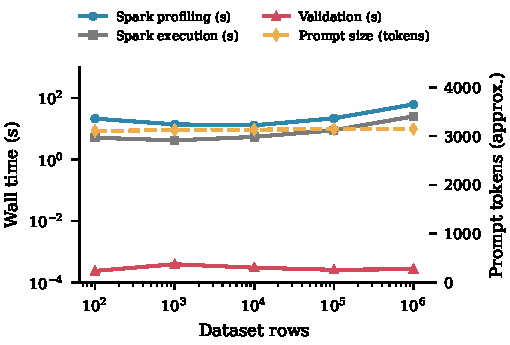
\includegraphics[width=\columnwidth]{scalability.pdf}
\caption{E3: Spark profiling and execution scale with data volume, whereas the AI-facing prompt and validation cost are independent of it (log--log; prompt size on the right axis).}
\label{fig:scale}
\end{figure}

\begin{table}[t]
\centering
\caption{E3 control-plane vs.\ data-plane cost by dataset size.}
\label{tab:scale}
\footnotesize
\setlength{\tabcolsep}{4pt}
\begin{tabular}{@{}rrrrrr@{}}
\toprule
\textbf{Rows} & \textbf{Profile (s)} & \textbf{Execute (s)} & \textbf{Prompt (chars)} & \textbf{Evid.} & \textbf{Validate (ms)}\\
\midrule
\tabinput{../tables/scalability.tex}
\bottomrule
\end{tabular}
\end{table}

\noindent\textbf{Scalability.} Fig.~\ref{fig:scale} and Table~\ref{tab:scale} report E3. Across four orders of magnitude ($10^2\to10^6$ rows, 6.4\,KB$\to$66\,MB), Spark profiling grew from $14$\,s to $62$\,s and plan execution from $4$\,s to $26$\,s (the $10^2$-row profiling time includes JVM warm-up). Over the same range the AI-facing prompt grew by only $1.4\%$ (12{,}423$\to$12{,}593 characters, $\approx$3.1k tokens; the growth is the extra digits in larger counts), the evidence bundle stayed at six items, and validating the six-recommendation plan took $0.24$--$0.40$\,ms regardless of size. This confirms the structural claim of \S\ref{sec:arch}: in CONVERGE the expensive, probabilistic component is invoked on $O(m+|E|)$ input, once per dataset, while the row-proportional work stays in the deterministic engine that was designed for it. A single model call of fixed cost can thus govern a cleaning job of arbitrary size, which is what makes LLM assistance economically compatible with big data workloads.
